
% !TEX root = ../presentation.tex


% |||||||||||||||||||||||
% ||||| Background ||||||
% |||||||||||||||||||||||

% \subsection{Background}



% \begin{frame}{Coverage}
%     % Concepts

%     % ~~~~\pcmd{usetheme}\p{[}\textit{theme options}\p{]}\ppar{UiO}
%     % \addtokomafont{descriptionlabel}{\normalfont\scshape}

%     {
%     % \newcommand{\boldLastStep}[1]{\only{\textbf{#1}}<4>}

%     % \newcommand{\fld}{\textsc}% field
%     \newcommand{\ths}{\textcolor{uioblue1}} % we will cover
   

%     \begin{description}[font=\scshape]
%         \item[\descItem{classical field theory} ]<1-> {perturbation theory}, {action principles}, \only{\ths}<4>{topological defects}
%         \item[\descItem{differential geometry} ]<2-> {pseudo-Riemannian manifolds}, conformal transformations, \only{\ths}<4>{hypersurfaces}%, tensor perturbations
%         \item[\descItem{modern cosmology} ]<3-> {concordance model}, \only{\ths}<4>{gravitational waves}
%     \end{description}


%     }
%     % \begin{itemize}
%     %     \item<1-> classical field theory
%     %     \item 
%     %     \item<2-> differential geometry
%     %     \item<3->
%     % \end{itemize}
%     % \begin{minipage}
%     % \end{minipage}
%     % \begin{tabular}{@{}lclc@{}}
%     %     \textbf{}
%     %     \dots & \dots \\
%     % \end{tabular}

% \end{frame}



\subsection{Gravitational physics}


\begin{frame}{Gravitational physics}
    %
    \uncover<1-2>
    {\newconcept{Newtonian mechanics} describe gravitation as an attractive force between massive objects.
    }\par\medskip
    \uncover<2->
    {In \newconcept{general relativity} (GR), gravitation is interpreted as an intrinsic property of spacetime curvature. %
    }%
    \uncover<3->
    {The existence of GWs is a consequence of GR. 
    }


    % \begin{description}[font=\scshape]
    %     \item[\descItem{\(+ \text{cosmological principle (CP)}\leadsto\)}]<3-> expanding universe; Friedmann--Lema\circumflex{i}tre--Robertson--Walker (FLRW) background
    %     \item[\descItem{\(+ \text{perturbations} \leadsto\)}]<4-> linearised gravity;
    % \end{description}
    % % \medskip
    % \uncover<3->{
    %     \begin{multline*}
    %         \text{GR} + \text{cosmological principle (CP)} \\ \leadsto \text{Friedmann--Lema\circumflex{i}tre--Robertson--Walker (FLRW) background} 
    %     \end{multline*}
    % % \small
    % % \[ \text{GR} + \text{cosmological principle (CP)}\leadsto \text{Friedmann--Lema\circumflex{i}tre--Robertson--Walker (FLRW) background} \]
    % }

    % % \smallskip
    % \uncover<4->{
    %     \begin{multline*}
    %         \text{GR} + \text{CP} + \text{perturbation theory} \\ \leadsto \text{cosmological perturbations} \supset \text{GWs}
    %     \end{multline*}
    % }
    % % \smallskip
    % \uncover<3->
    % {The existence of \newconcept{gravitational waves} (GWs) is a consequence of GR. 
    % }%\note<3>{A concequence of this is GWs, which do not have a non-relativistic analogy. \par}
    % \par\medskip
    % \uncover<4->
    % {Applying the cosmological principle (CP) to GR, we get the Friedmann equations that governs the expansion of the universe, and in turn the standard model of cosmology known as the \newconcept{\textLambda{}CDM model}.
    % }%\note<4>{Also born from GR is modern cosmology.\par}

    % % \begin{itemize}
    % %     % \item<2-> What is GR? %\citep{adamekGeneralRelativityCosmic2016}
    % %     % \item<2-> What are GWs?
    % %     \item<2-> Symmetron?
    % %     \item<2-> Hubble tension + PTAs
    % % \end{itemize}
    % % \thelinewidth

% *************************************
% NOTES *******************************
\begin{notes}[2][gravitation]
    \nnote{1}{}
    \itnote{2}{
        \item Also born from GR is modern cosmology.
    }
    \itnote{3}{
        \item A consequence of this is GWs, which do not have a non-relativistic analogy. (No GWs ``at home'')
        \item Conceptually complicated
        \item Will not dig into the formalities of GWs 
    }
\end{notes}
% *************************************

\end{frame}


\begin{frame}{General relativity}
    % Metric $g\_{\mu\nu}$
    Curvature of spacetime manifold $\mathscr{M}$ is described by
    \begin{equation}
        \overbrace{{ds}^2}^{\text{line element}} = \overbrace{g\_{\mu\nu}}^{\text{metric}} {\diff x\^\mu} {\diff x\^\nu}.
    \end{equation}
    The components obey the Einstein equations:
    \begin{equation}
        \mathcal{G}\_{\mu\nu} = 8\piGN T\_{\mu\nu}.
    \end{equation}

    \only<1>{%
    \begin{textblock*}{\textwidth}(1cm,0.7\paperheight)
        \ifOnlyNotes\else
        {\small\color{paletaupe}{%
        Here, $\mathcal{G}\_{\mu\nu}= \mathcal{R}\_{\mu\nu}- g\_{\mu\nu}\mathcal{R}/2$ is the Einstein tensor, $\mathcal{R}\_{\mu\nu}$ ($\mathcal{R}$) the Ricci tensor (scalar), and $T\_{\mu\nu}$ the stress--energy (SE) tensor.}
        }\fi
    \end{textblock*}
    }

    
    % \note<2>{We mention two solutions to this equation when there are one time dimension and three spatial dimensions.\par}
    \uncover<2->{
    \medskip

    \fcolorbox{uioorange3}{white}{\paragraph{Special relativity.}
    $g\_{\mu\nu}= \eta\_{\mu\nu} = \text{diag}(-1,+1, +1, +1)= \text{Minkowski metric}$ }
    \smallskip
    
    \fcolorbox{uiopink2}{white}{\paragraph{Flat, expanding universe.}
    $g\_{\mu\nu}= a^2(x\^0 )\eta\_{\mu\nu}= \text{(flat) FLRW metric}$ }
    
    }



% *************************************
% NOTES *******************************
\begin{notes}[2][GR]
    \nnote{1}{``Spacetime tells matter how to move; matter tells spacetime how to curve.'' ---John Wheeler}
    \nnote{2}{We mention two solutions to this equation when there are one time dimension and three spatial dimensions.}
\end{notes}
% *************************************


\end{frame}


\begin{frame}{\textit{Quick look}: Metric perturbations}
    Under $g\_{\mu\nu} \to \pert{g}\_{\mu\nu} = g\_{\mu\nu} + \delta  g\_{\mu\nu} $, we get the linearised Einstein equations
    \begin{equation}
        \pert{\mathcal{G}}\_{\mu\nu} = 8\piGN \pert{T}\_{\mu\nu}.
    \end{equation}


    \medskip


    \fcolorbox{uioorange3}{white}{\paragraph{Minkowski.}
    $\pert{g}\_{\mu\nu}= \eta\_{\mu\nu} + h\_{\mu\nu}$ }%
    \uncover<2>{
    {\color{O3}
        \(\,\dots \twoheadrightarrow \, \) \(\sq\nped{M} h\_{ij} \propto T\_{ij} \)
    }}

    % \uncover<2>{
    %     \smallskip
    %     {\color{O3}
    %     \(\dots \twoheadrightarrow \quad\) \(\sq\nped{M} h\_{ij} \propto T\_{ij} \)
    % }}
    
    \smallskip
    
    \fcolorbox{uiopink2}{white}{\paragraph{Flat FLRW.}
    $\pert{g}\_{\mu\nu}= a^2(x\^0 )\bclosed{\eta\_{\mu\nu} + h\_{\mu\nu}}$ }%
    \uncover<2>{
    {
        \color{R2}
    \(\,\dots \twoheadrightarrow \,\) \(\sq h\_{ij} \propto a^{-2}T\_{ij} \)%, a.k.a. GWs!
    }}


    % \uncover<3>{
    %     \begin{equation}
    %         \sq h
    %     \end{equation}
    % }



    % \uncover<2>{
    %     \smallskip
    %     {\color{R2}
    %     \(\dots \twoheadrightarrow \quad\) \(\sq h\_{ij} \propto a^{-2}T\_{ij} \)%, a.k.a. GWs!
    % }}


% *************************************
% NOTES *******************************
\begin{notes}[2][GWs]
    \nnote{1}{Before we move on: Quick look; how this relates to GWs.}
    \itnote{2}{
        \item \textcolor{O1}{Choose coords. s.t.}
        \item EOM for GWs in expanding spacetime!
        \item Inhomogeneous (damped) wave eq.
        \item 2 physical dofs >> 2 polarisations
        \item Unlike density perturbations, there is no Newtonian analogy to GWs (other words: conceptually complicated)
        }
\end{notes}
% *************************************
\end{frame}





\subsection{Cosmology}

\begin{frame}{Background cosmology}

    \textcolor{black}{
    \paragraph{Cosmological principle.}%
    \textit{The universe is homogeneous and isotropic.}}
    \medskip

    \uncover<2->{\small%
    Model universe from perfect fluids $s$ with equation of state (e.o.s.) $p_s = w_s \rho_s$. Hubble parameter is}
    \uncover<2->{
        \begin{columns}
            \begin{column}{0.2\textwidth}
                \uncover<3->{\centering\adjincludegraphics[width=\columnwidth, keepaspectratio, trim={{0.1\width} {0.14\height} {0.1\width} {0.1\height}}, clip]{figs/lcdm_pie.png}
                \centering\footnotesize%
                \textcolor{uiogrey}{(today)}}
            \end{column}
            %
            \begin{column}{0.76\textwidth}\small
                % Model universe from perfect fluids $s$ with equation of state (e.o.s.) $p_s = w_s \rho_s$. Hubble parameter is
                {
                \only<1-3>{\newcommand{\Hnot}{\mathcolor{black}{H_0}}}
                \only<4>{\newcommand{\Hnot}{\mathcolor{R1}{H_0}}}
                %
                \uncover<2->{\begin{equation}
                    H^2(a) = \Hnot^2 
                    \sum_{s}\Omega_{s0}a^{-3(1+w_s)} \uncover<1-2>{.}\uncover<3->{= \Hnot^2\, \pclosed{ \Omega\ped{m0}a^{-3} + \Omega\ped{de0} }.}
                \end{equation}}
                }
                \uncover<3->{\medskip
                \paragraph{\textcolor{G2}{\textLambda{}}\textcolor{B2}{CDM}.} \textcolor{G2}{Dark energy (DE) $\leftrightarrow$ a cosmological constant (\textLambda)} $+$ \textcolor{O2}{baryonic} \& \textcolor{B2}{cold dark matter (CDM)}.}
            \end{column}
            %
        \end{columns}   

    }




% *************************************
% NOTES *******************************
\begin{notes}[4][cosmology]
    \nnote{1}{Earth not at privileged position}
    \nnote{2}{The negative pressure of the former is responsible for the current accelerated expansion of the universe, given by the value of the Hubble constant $H_0$.}
    \nnote{3}{}
    \nnote{4}{GR very precise in e.g. solar systems, but there are problems in modern cosmology; one of them has to do with this constant}
\end{notes}
% *************************************


\end{frame}



\begin{frame}

    % \medskip
    \uncover<1->{\aProblem{\(\bullet \)Hubble tension.}{%
        There is a discrepancy between measurements of the Hubble constant $H_0 = 100\text{h} \unit{km}\unit{s}^{-1}\unit{Mpc}^{-1}$:
        \begin{align*}
            \text{``Late universe'' measurements} &\leadsto \text{h} \sim 0.73 \mathcolor{uiogrey}{\pm 0.02} \\
            \text{``Early universe'' measurements} &\leadsto \text{h} \sim 0.67 \mathcolor{uiogrey}{\pm 0.01} 
        \end{align*}
    }}%
    \uncover<2->{\aSolution{\(\bullet\)possible solution.}{
        A common work-around is to let DE have time-dependent e.o.s. parameter $w\ped{de}= w\ped{de}(a)$, which can be ensured by a dynamical scalar field $\phi$ (cf.~(a)\fcolorbox{white}{B3}{\textcolor{black}{\textbf{symmetron}}},\invisible<1>{\footnote<2>{\cite{hinterbichlerSymmetronCosmology2011,perivolaropoulosGravitationalTransitionsExplicitly2022}}} quintessence, phantom dark energy).%
        % \textcolor<3>{white}{phantom dark energy).}\par\textcolor<2>{white}{phantom dark energy).}
    }}
    % \only<3>{\ifOnlyNotes\else
    %     \begin{textblock*}{0.6\paperwidth}(0.36\paperwidth, 0.61\paperheight)
    %         \includegraphics[keepaspectratio,height=0.39\paperheight]{figs/symmetron_screen_milky.png}
    %     \end{textblock*}\fi
    % }


% *************************************
% NOTES *******************************
\begin{notes}[2][Hubble tension]
    \itnote{1}{
        \item There are problems, but will only address the phenomenologically indifferent accelerated expansion of the universe \emph{today}.
        \item direct (distance ladder) vs. indirect (CMB experiments)
        \item More precise measurements (about a decade ago) gives no overlap between uncertainties.
    }
    \itnote{2}{
        \item Often associated with a PT, which in turn can imply the existence of topological defects.
        \item Motivates models s.a. scalar-field theories
        \item Symmetron: fifth force mediated when symmetry is broken (low-density vacuum)
        \item GR accurate in laboratories---fifth force must be screened here
    }
    % \nnote{3}{Now in a universe, }
\end{notes}
% *************************************
\end{frame}


% \begin{frame}{Auxiliary fields}
%     % Common work-around: change $w\ped{de}=w\ped{\textLambda}$ to $w\ped{de}=w_{\phi}(a)$

%     % Can be obtained by introducing a scalar field $\phi$

%     \medskip
%     If the Lagrangian inhabits a spontaneously broken symmetry, a phase transition can occur if exterior criteria are met, and topological defects may form.

% \end{frame}

% \begin{frame}{Topological defects}
    
% \end{frame}

% \begin{frame}{Metric perturbations}

%     If $g\_{\mu\nu}$ is a solution to Einstein's equation, we find the corresponding linearised Einstein's equation by adding a small perturbation to the metric:
%     \begin{equation}
%         g\_{\mu\nu}\to \pert{g}\_{\mu\nu} = g\_{\mu\nu} + \delta g\_{\mu\nu}, \quad \abs{\delta g\_{\mu\nu}}\ll\abs{g\_{\mu\nu}}.
%     \end{equation}
%     Now, $\pert{\mathcal{G}}\_{\mu\nu} = 8\piGN \pert{T}\_{\mu\nu}$ is the linearised Einstein equation, to be solved orderly.% where the dot signifies the perturbed quantity.

%     \medskip
%     \uncover<2->{%\fcolorbox{R2}{white}{%
%     \paragraph{Cosmological perturbation theory.}%
%     $\pert{g}\_{\mu\nu}=a^2 \pclosed*{ \eta\_{\mu\nu}  + h\_{\mu\nu} }$ is subject to a scalar--vector--tensor (SVT) decomposition. % Solving the linearised 
%     % }
%     }
%     \note<2->{Expansion causes a damping term to the wave equation}
    


%     % At background level, CP holds, and we have $g\_{\mu\nu}= a^2 (\tau) \eta\_{\mu\nu}$, where $\tau=x\^0$ is conformal time. 
%     % \smallskip
%     % \uncover<2->{Structure formation due to small primordial field variations that during inflation blows up.}
%     % \medskip
%     % \uncover<3->{}

% \end{frame}





\subsection{Phase transitions}

% \begin{frame}{Cosmic phase transition}
%     The \newconcept{symmetron model}\footnote{Asymmetron~\citep{perivolaropoulosGravitationalTransitionsExplicitly2022} is a generalisation of symmetron~\citep{hinterbichlerSymmetronCosmology2011}.} is characterised by the following:
%     \smallskip
%     \begin{itemize}
%         \item<1-> Sombrero potenital in vacuum, \(V(\phi) = \lambda\phi^4/4 - \mu^2\phi^2/2\).
%         \begin{itemize}
%             \item Two vacuum states.
%             \item Symmetry under $\phi \to -\phi$.
%         \end{itemize}
%         \item<2-> Coupling to matter induces cosmic phase transition (PT).
%         \begin{itemize}
%             \item Convenient to use the \newconcept{effective potential} $V\ped{eff}(\phi)$, s.t. the equation of motion (e.o.m.) for $\phi$ reads $\sq \phi = \partial_\phi V\ped{eff}(\phi)$.
%             \item Vacuum expectation value (VEV) different before and after PT.
%             \item Domain walls form during discrete-symmetry breaking.
%         \end{itemize}

%     \end{itemize}

% % *************************************
% % NOTES *******************************
% \begin{notes}{8}
    
% \end{notes}
% % *************************************
% \end{frame}



% \begin{frame}{Symmetron phase transition}
%     %
%     % \fcolorbox{G2}{white}{
%     %     \parbox{\textwidth}{
%     %         \begin{raggedright}
%     %             \small
%     %             Total action: $S = S\nped{EH} + S_{(\phi)} + S\ped{(m)}$, with $\mathcal{L}_{(\phi)}= X(\phi)- V(\phi)$ 
%     %         \end{raggedright}
%     %         }
%     % }
%     % \medskip

%     Symmetron\citef{hinterbichlerSymmetronCosmology2011} (or generalisation asymmetron\citef{perivolaropoulosGravitationalTransitionsExplicitly2022}) characterised by sombrero potential in vacuum. 
%     \smallskip



%     Sombrero potential in vacuum. Coupling to matter induces a first-order phase transition 

%     % \note{Describe with example.}

%     % The total action is $S = S\nped{EH} + S_{(\phi)} + S\ped{(m)}$, with $\mathcal{L}_{(\phi)}= X(\phi)- V(\phi)$. 

%     % \medskip
%     % \paragraph{Example.}%
%     % Symmetron\citef{hinterbichlerSymmetronCosmology2011} (or generalisation asymmetron\citef{perivolaropoulosGravitationalTransitionsExplicitly2022}) with sombrero potential; $V(\phi) = \lambda\phi^4/4 - \mu^2\phi^2/2$. 

%     % The action for a scalar field $\phi$ in curved spacetime is 
%     % \begin{equation}
%     %     S = \only<1>{S\nped{EH} + S_{(\phi)}}
%     %     \only<2->{\integ[4]{x} \sqrt{-g}\bclosed{ M\nped{Pl}^2\mathcal{R}/2 + X(\phi) - V(\phi) }} 
%     %     + S\ped{(m)}
%     % \end{equation}
%     \note<1>{Note that regular GR is retrieved when middle term is zero.}


%     % \comment{effective potential, PT, defect formation}

%     % Symmetron\citef{hinterbichlerSymmetronCosmology2011}, and Asymmetron\citef{perivolaropoulosGravitationalTransitionsExplicitly2022}



% \end{frame}


% \begin{frame}{Symmetron}
%     Mexican-hat potential
%     \begin{equation}
%         V(\phi) = \frac{\lambda}{4}\phi^4 - \frac{\mu^2}{2}\phi^2
%     \end{equation}

%     % \only<2>{\begin{textblock*}{0.6\textwidth}(0.5\textwidth,1cm)
%     %     \includegraphics[width=\columnwidth]{../../figs/Background/symmetron_screen_milky.png}
%     % \end{textblock*}}
% \end{frame}




% \uiofullpageimage{figs/dw_pt1.png}

% \begin{frame}{Symmetron}
%     The symmetron model\citef{hinterbichlerSymmetronCosmology2011}

%     \medskip
%     Asymmetron\citef{perivolaropoulosGravitationalTransitionsExplicitly2022}
% \end{frame}

% \begin{uioimageframe}[info={$a_\ast = 0.33$, $\xi_\ast = 3.33\times 10^{-4}$, \only<1>{$\beta_\ast=1$}\only<2>{$\beta_+ = 1.1$, $\beta_-=0.9$}}]{gifs/asym/asym-99.png}
%     The \uncover<2>{\textcolor{G2}{a}}\textcolor{B2}{symmetron} effective potential is
%     \begin{multline}
%         V\ped{eff}(\phi) = \frac{\lambda}{4}\phi^4 \uncover<2>{\mathcolor{G2}{-\frac{\kappa}{3}\phi^3}} 
%         + \frac{\mu^2}{2} \pclosed{\upsilon-1}\phi^2,
%     \end{multline}
%     where $\upsilon\equiv \pclosed*{a_\ast/a}^3$.
% \end{uioimageframe}


\begin{frame}[plain]%{%
    % \only<1>{Symmetron}%
    % \only<2>{Asymmetron}}
    % \animategraphics[loop, controls, width=0.6\textwidth, autoplay]{10}{gifs/asym/asym-}{0}{99}
    \begin{columns}   
    % \medskip 
    \begin{column}{0.5\textwidth}\small
        
        The \uncover<2>{\textcolor{G2}{a}}\textcolor{B2}{symmetron} %\footnote{\textcolor{B3}{\cite{hinterbichlerSymmetronCosmology2011}}}\uncover<2>{\footnote{\textcolor{G3}{\cite{perivolaropoulosGravitationalTransitionsExplicitly2022}}}}
        effective potential is
        \begin{multline}
            V\ped{eff}(\phi) = \frac{\lambda}{4}\phi^4 \uncover<2>{\mathcolor{G2}{-\frac{\kappa}{3}\phi^3}} 
            + \frac{\mu^2}{2} \pclosed{\upsilon-1}\phi^2,
        \end{multline}
        where $\upsilon\equiv \rho\ped{(m)}/\rho_\ast \simeq \pclosed*{a_\ast/a}^3$.%~\textcolor{B3}{\citep{hinterbichlerSymmetronCosmology2011}}\uncover<2>{~\textcolor{G3}{\citep{perivolaropoulosGravitationalTransitionsExplicitly2022}}}

        \medskip
        \textcolor{paletaupe}{Symmetry breaking at critical density $\rho_\ast$.}
    \end{column}
    \begin{column}{0.5\textwidth}\small
        % 
        \centering
        \vspace*{-3mm}
        % ****** ANIMATION ******
        \ifCompAnims
            \animategraphics[loop,keepaspectratio,width=\columnwidth,height=0.99\textheight,autoplay]{20}{gifs/asym/asym-}{0}{99}%{99}
        \else
            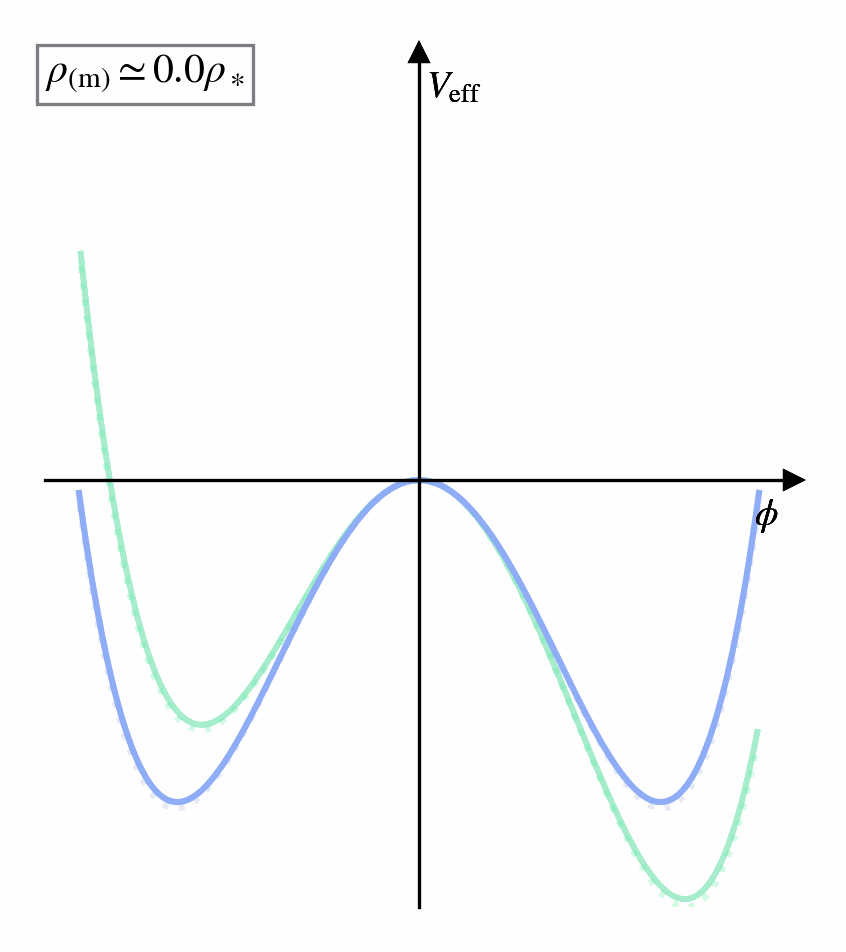
\includegraphics[keepaspectratio,width=\columnwidth,height=0.98\textheight]{gifs/asym/asym-99}
        \fi
        % ***********************
        % TMP:
        % 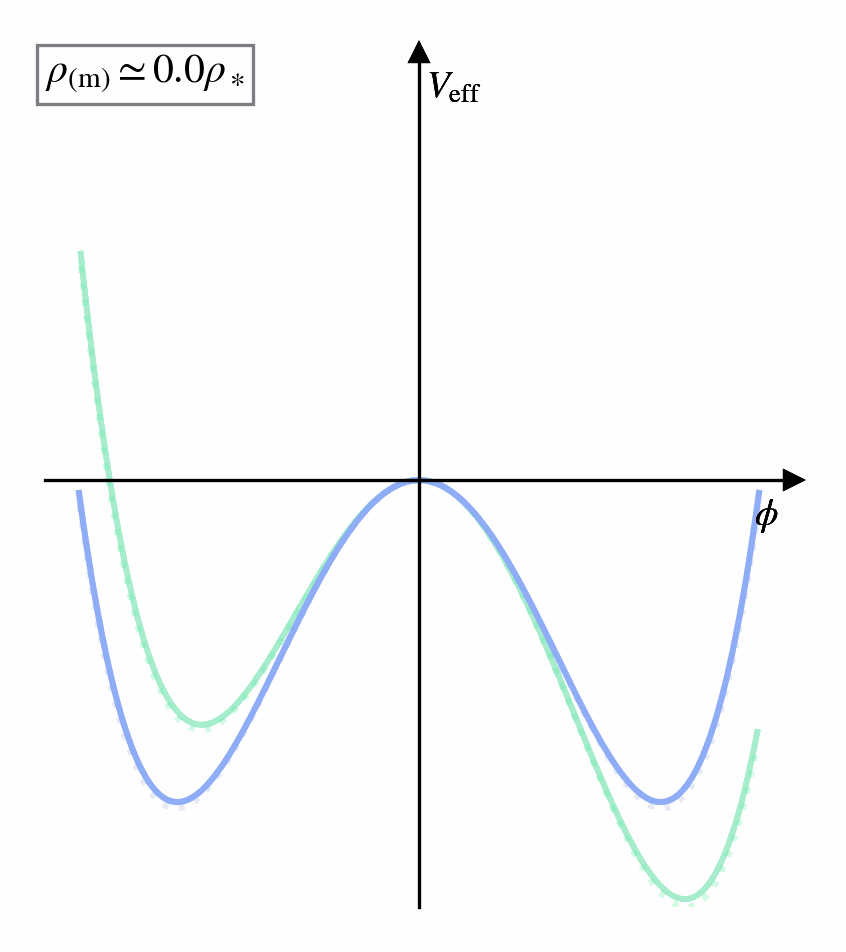
\includegraphics[keepaspectratio,width=\columnwidth,height=0.98\textheight]{gifs/asym/asym-99}%
        % -
        % \rlap{\hspace*{1mm}\rotatebox{90}{\scriptsize {$a_\ast = 0.33$, $\xi_\ast = 3.33\times 10^{-4}$}}}\par
    \end{column}
    \end{columns}
    % \uiobegincolumns
    % \movie[externalviewer]{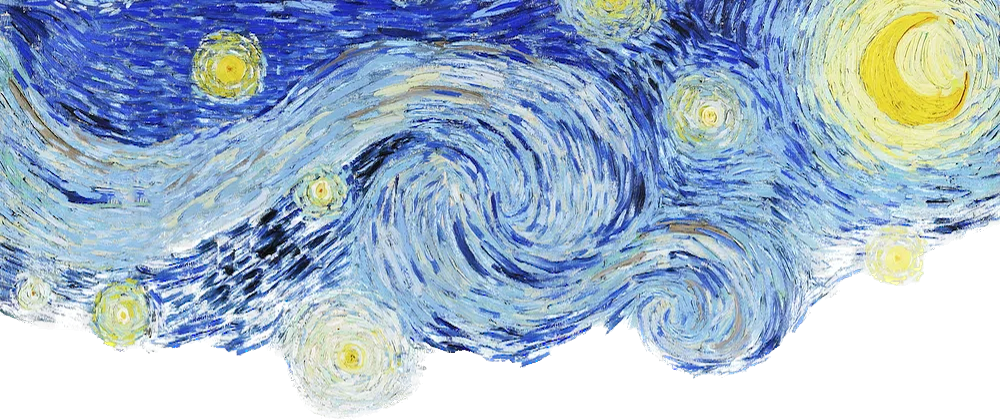
\includegraphics[width=1.0\textwidth]{starry-night.png}}{ani_achi.mp4}



% *************************************
% NOTES *******************************
\begin{notes}[2][symmetron PT]
    \itnote{1}{
        \item Use an effective potential to describe the phase transition.
        \item Here, scale factor and energy density are the used ``synonymously'' (for our purposes, anim with time)
        \item coupling to matter restores symmetry in dense regions
    }
    \nnote{2}{\dots which is an attempt at solving a different problem, which we will get back to}
\end{notes}
% *************************************
\end{frame}










\begin{frame}[plain,fragile]
    \ifOnlyNotes
    \only<1-3>{}
    \else
    \begin{textblock*}{\paperwidth}(0cm,0cm)
        \foreach \x in {1,...,3}{
                \only<\x>
                {\adjincludegraphics%
                [width=\paperwidth,trim={0 {0.02\height} 0 {0.02\height}},clip]%
                {figs/dw_pt\x.png}}
                % {\includegraphics{width=\paperwidth,height=\paperheight}{figs/dw_pt\x.png}}
        }%
    \end{textblock*}
    %
    % \fi
    
    \only<1-3>{\begin{textblock*}{3cm}(0.29\textwidth,0.38\textheight)
        % \Large \fcolorbox{uiogrey}{uiogrey}{\textcolor{R3}{\(\phi\only<1>{\gtrsim 0}\only<2>{> 0}\only<3>{=\phi_+} \)}}
        \Large \(\phi\only<1>{\gtrsim 0}\only<2>{> 0}\only<3>{=\phi_+} \)
    \end{textblock*}

    \begin{textblock*}{3cm}(0.76\textwidth,0.21\textheight)
        \Large \(\phi\only<1>{\lesssim 0}\only<2>{< 0}\only<3>{=\phi_-} \)
    \end{textblock*}

    \begin{textblock*}{3cm}(0.32\textwidth,0.83\textheight)
        \Large \(\phi\only<1>{\simeq 0}\only<2>{= 0}\only<3>{=0} \)
    \end{textblock*}}
    \fi

    % \only<4->{
    %     \begin{textblock*}{0.5\paperwidth}(0.4\paperwidth, 0.06\paperheight)
    %         \fcolorbox{white}{white}{
    %             \parbox{0.5\paperwidth}{
    %                 \uncover<2->{\aProblem{\(*\)overclosing problem.}{A DW network modelled as a perfect fluid will have e.o.s.-parameter $w\ped{dw}=-2/3$. As contributor to the total energy budget of the universe, it would quickly dominate.}
    %                 }
    %                 \uncover<3->{%
    %                     \aSolution{\(*\)proposed solutions.}{Slightly broken vacuum degeneracy; $V(\phi_+) \neq V(\phi_-)$ (e.g.~asymmetron), or let walls melt away.}
    %                 }
    %             }
    %         }
    %     \end{textblock*}
    % }


% *************************************
% NOTES *******************************
\begin{notes}[3]
    \nnote{1}{At PT, random fluctuations around (yellow) vacuum state}
    \nnote{2}{Shortly after}
    \nnote{3}{Infinitely long after >> domain walls (in truth: fluctuations)}
    % \nnote{4}{Briefly mention the problem, and thus motivate models with time-dependent surface tension or non-degenerate vacua}
\end{notes}

% *************************************
\end{frame}



% \begin{frame}[plain]%{%
%     \begin{columns}   
%     \begin{column}{0.5\textwidth}\small
%         The scalar field $\phi$ will oscillate around the true minima $\phi_\pm$ \comment{animation:pause and zoom in}
%     \end{column}
%     \begin{column}{0.5\textwidth}\small
%         % 
%         \centering
%         \vspace*{-3mm}
%         % ****** ANIMATION ******
%         % \animategraphics[loop,keepaspectratio,width=\columnwidth,height=0.99\textheight,autoplay]{5}{gifs/asym_ball/asym_ball-}{0}{199}
%         % (tmp)
%         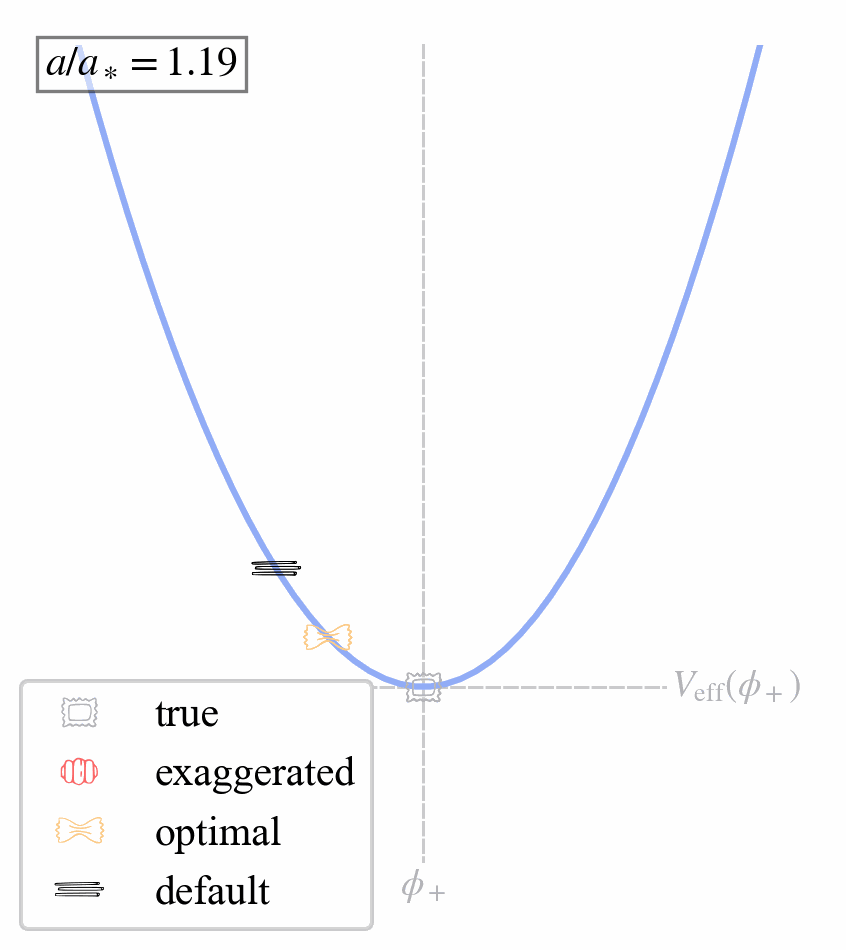
\includegraphics[keepaspectratio,width=\columnwidth,height=0.98\textheight]{gifs/asym_ball/asym_ball-199}
%         % ***********************
%         % \rlap{\hspace*{1mm}\rotatebox{90}{\scriptsize {$a_\ast = 0.33$, $\xi_\ast = 3.33\times 10^{-4}$}}}\par
%     \end{column}
%     \end{columns}
    
% \end{frame}

% \begin{uioanimframe}[info={?}]{gifs/asym/asym-0}%{0}{99}
%    {Helo}
% \end{uioanimframe}

% \subsection{Topological defects}

% \begin{frame}{\unfinishedSlide~Domain walls} %{Topological defects}
%     % \uncover<1->{Symmetry breaking \comment{blahblah defects}. }
%     % \uncover<2>{\newconcept{Domain walls} (DWs) are two-dimensional\note{spatial dimensions} topological defects }
%     A symmetry-breaking phase transition may lead to the formation of \newconcept{topological defects}. 

%     \comment{FIXME}

%     % The symmetry decides the defect; discrete symmetry lead to domain

%     Breaking of a discrete symmetry in four-dimensional spacetime, such as invariance under $\phi \to -\phi$, leads to the formation of domain walls. 

%     \bigskip
%     \uncover<2->{\aProblem{\(*\)overclosing problem.}{A DW network modelled as a perfect fluid will have e.o.s.-parameter $w\ped{dw}=-2/3$. As contributor to the total energy budget of the universe, it would quickly dominate.}
%     }
%     \uncover<3->{%
%         \aSolution{\(*\)proposed solutions.}{Slightly broken vacuum degeneracy; $V(\phi_+) \neq V(\phi_-)$ (e.g.~asymmetron), or let walls melt away.}
%     }


% % *************************************
% % NOTES *******************************
% \begin{notes}{10}
    
% \end{notes}
% % *************************************


    
% \end{frame}






% \subsection{Gravitational waves}

\begin{frame}{The domain-wall ripple effect}


    % Domain walls are candidate sources for the GW signal in the \textit{NANOGrav 15 yr} dataset.

    % \( g\_{\mu\nu} \to g\_{\mu\nu} + \delta g\_{\mu\nu} \)

    GWs from DWs are expected to be within reach of future experiments. 

    % Pulsar Timing Arrays (PTAs) provide \comment{\dots}

    \bigskip


    % Recent PTA observations \dots 



    % \comment{FIXME}



    % In fact, domain-wall models have recently been constrained from the \textit{NANOGrav 15 yr} data set.


    % > OVERCLOSING PROBLEM


    \uncover<2->{%
        \aProblem{\(*\)overclosing problem.}{A DW network modelled as a perfect fluid will have e.o.s.-parameter $w\ped{dw}=-2/3$. As contributor to the total energy budget of the universe, it would quickly dominate.}
    }
    \uncover<3->{%
        \aSolution{\(*\)proposed solutions.}{Slightly broken vacuum degeneracy; $V(\phi_+) \neq V(\phi_-)$ (e.g.~asymmetron), or let walls melt away.}
    }


    % \comment{cosmological constraints on PTs, }
    

% *************************************
% NOTES *******************************
\begin{notes}[3]
    \itnote{1}{
        \item DW models can be constrained by PTA observations.
        \item Colliding, collapsing, decaying, stochastic fluctuations
        \item We will look at planar DWs formed during late-time PT in a matter-dominated universe, and specifically how a spatial perturbation can induce GWs
    }
    \nnote{2}{Mention a problem\dots}
    \nnote{3}{Motivation for asymm, and emphasise the usefulness of considering time-dep. surface tension}
\end{notes}
% *************************************
\end{frame}



% \begin{frame}{Gravitational waves}
%     % \note{Fast forward \dots\par}
%     We take the background geometry to be FLRW and consider only perturbations in the tensor sector. The perturbed line element reads
%     \begin{equation}
%         \pert{ds}^2 = a^2(\tau) \bclosed{ -{\diff \tau}^2 + \pclosed*{\Krondelta{_{ij}} + h\_{ij}} {\diff x\^i}{\diff x\^j} } 
%     \end{equation}
%     and the e.o.m. for \( \only<1>{h\_{ij}(\tau, \vec{x})}  \only<2>{\tilde{h}_P(\tau, \vec{k})} \) reads
%     %linearised Einstein equation reduces to
%     \begin{equation}
%         \only<1>{\sq h\_{ij} = -16\piGN \pi\_{ij},}
%         \only<2>{\ddot{\tilde{h}}_P + 2\mathcal{H} \dot{\tilde{h}}_P + k^2 \tilde{h}_P = 16\piGN a^2 \tilde{\pi}_P, }
%     \end{equation}
%     where \only<1>{${\pi\_{ij}}$ is the transverse and traceless (TT) part of $T\iud{i}{j}$.}%
%     \only<2>{$\tilde{\pi}_P$, $P=+, \times$, is the $P$-polarised part of $\tilde{T}\iud{i}{j}$.}

% % *************************************
% % NOTES *******************************
% \begin{notes}[2][\textcolor{G2}{SKIP?}]
%     \itnote{1}{
%         \item Short story: 2 tensor dofs \dots 
%     }
%     \itnote{2}{
%         \item Fourier space
%         \item 2 pols = 2 dofs $\to$ How they affect a ring of test particles.
%         \item $\Rightarrow$ Now, with this background, we may move on to the actual project.
%         }
% \end{notes}
% % *************************************
% \end{frame}


% \begin{frame}{Gravitational waves \uncover<2>{\textcolor{R2}{in flat, expanding universe}}}
%     \uncover<1->{
%         Perturbations to the background metric are \comment{\dots}
%         \begin{equation}
%             \pert{g}\_{\mu\nu} = 
%             {g\_{\mu\nu} + \delta g\_{\mu\nu}}
%             \uncover<2>{\mathcolor{R2}{=a^2 \pclosed*{ \eta\_{\mu\nu}  + h\_{\mu\nu} }}}.
%         \end{equation}
%     }%
%     \uncover<2->{The linearised Einstein equations, \( \pert{\mathcal{G}}\_{\mu\nu} = 8\piGN \pert{T}\_{\mu\nu} \), reduce to 
%     \begin{equation}
%         \sq h\_{ij} = -16\piGN \pi\_{ij}
%     \end{equation}
%     in the \newconcept{transeverse--traceless} (TT) gauge.
%     }


%     \medskip
%     \uncover<3->{\paragraph{Sources.}%
%     % Black-hole (BH) mergers,
%     Massive binaries (2015), 
%     }
%     \uncover<3->{gravitational wave background (GWB) (2023)}

%     % \comment{$f\ped{yr} \equiv 1\unit{year}^{-1}\approx 31.7 \unit{nHz}$}
    
% \end{frame}


% \begin{frame}{Gravitational-wave observations}
%     \note{We will not go through the various methods of GW observations.}
%     \uncover<1->{
%         There are various 
%     }
% \end{frame}


% \begin{frame}{Observations and implications}
    

%     Recent PTA observations \dots
% \end{frame}



% \uiobigimage{Pulsar Timing Arrays \comment{remove?}}{figs/Detnoise_summary_plot.png}{Credit: \href{https://nanograv.org/15yr/Summary/Detector}{Shami Chatterjee/NANOGrav}}
% \url{https://nanograv.org/15yr/Summary/Detector}

% \begin{frame}{New physics}
%     About GWs as probe for new physics

% \end{frame}






